\section{Wielomian Jonesa} % (fold)


Relacja kłębiasta okazała się być kluczem do sukcesu w poszukiwaniu nowych niezmienników wielomianowych.
Vaughan Jones, matematyk nowozelandzki, zaprezentował w~roku 1984 nowy niezmiennik splotów jako produkt uboczny podczas pracy nad algebrami operatorowymi, które nas nie interesują.
Był to przełomowy rezultat, a~już cztery miesiące później ogłoszono znalezienie jeszcze bardziej wyrafinowanego niezmiennika, któremu przyjrzymy się w~kolejnej sekcji.

Aby lepiej zrozumieć wielomian Jonesa, zbadamy najpierw nieco prostszy obiekt, nawias Kauffmana.
Później zajmiemy się węzłami alternującymi.

\subsection{Definicja kombinatoryczna -- klamra Kauffmana} % (fold)
\label{sub:kauffman_bracket}
Klamra Kauffmana to wielomian Laurenta jednej zmiennej zdefiniowany w pracy \cite{kauffman87} z 1987 roku, oparty na ruchach Reidemeistera.
Dzięki swojej prostocie mógł być odkryty na początku XX wieku, nim jeszcze maszyneria teorii węzłów została rozwinięta.

Poszukujemy niezmiennika dla splotów o~kilku prostych własnościach.
Przede wszystkim żądamy, by niewęzłowi przypisany był wielomian $1$: $\bracket{\LittleUnknot} = 1$.
Po drugie chcemy wyznaczać nawiasy znając je dla prostszych splotów, co zapiszemy symbolicznie $\bracket{\LittleRightCrossing} = A \bracket{\LittleRightSmoothing} + B \bracket{\LittleLeftSmoothing}$.
Zależy nam wreszcie na tym, by móc dodać do splotu trywialną składową: $\langle L \cup \LittleUnknot \rangle = C \langle L \rangle$.
Prosty rachunek pokazuje wpływ drugiego ruchu Reidemeistera na klamrę:
\begin{equation}
    \bracket{\reidemeisterIIaa}
    = (A^2 + ABC + B^2) \bracket{\LittleLeftSmoothing} + BA \bracket{\LittleRightSmoothing}
    \stackrel{?}{=} \bracket{\LittleRightSmoothing}.
\end{equation}

Aby zachodziła ostatnia równość wystarczy przyjąć $B = A^{-1}$, co wymusza na nas wartość trzeciego parametru: $C = -A^2 - A^{-2}$.
W ten sposób odkryliśmy definicję.

\begin{definition}[klamra Kauffmana]
    \index{klamra!Kauffmana}
    \label{def:kauffman_bracket}
    Wielomian Laurenta $\bracket{D}$ dla diagramu splotu $D$ zmiennej $A$,
    który jest niezmienniczy ze względu na gładkie deformacje diagramu,
    a~przy tym spełnia trzy poniższe aksjomaty:
    \begin{align}
        \bracket{\LittleUnknot} & = 1 \\
        \bracket{D \sqcup \LittleUnknot} & = (-A^{-2} - A^2) \bracket{D} \\
        \bracket{\LittleRightCrossing} & = A \bracket{\LittleRightSmoothing} + A^{-1} \bracket{\LittleLeftSmoothing}
    \end{align}
    nazywamy klamrą Kauffmana.
\end{definition}

Tutaj $\LittleUnknot$ oznacza standardowy diagram dla niewęzła,
zaś trzy symbole $\LittleRightCrossing$, $\LittleRightSmoothing$ oraz $\LittleLeftSmoothing$ odnoszą się do diagramów,
które są identyczne wszędzie poza małym obszarem (tak jak w~relacji kłębiastej).
\textbf{Duplikat wyjaśnienia, czym jest relacja kłębiasta?}
Diagramy $\LittleRightSmoothing$ oraz $\LittleLeftSmoothing$ nazywa się odpowiednio
dodatnim (prawym) i~ujemnym (lewym) wygładzeniem $\LittleRightCrossing$.

\begin{lemma}
    Klamra Kauffmana każdego diagramu wyznacza się w~skończenie wielu krokach.
\end{lemma}

\begin{proof}
    Jeżeli diagram $D$ ma $n$ skrzyżowań, to nieustanne stosowanie aksjomatu trzeciego pozwala na zapisanie $\bracket{D}$ jako sumy $2^n$ składników,
    z~których każdy jest po prostu zamkniętą krzywą i~ma trywialną klamrę ($\bracket{\LittleUnknot} = 1$).
    Klamrę sumy wyznacza się korzystając z~drugiego aksjomatu.
\end{proof}

Przedstawimy teraz wpływ ruchów Reidemeistera na nasz nowy wielomian.

\begin{lemma}
    Drugi i~trzeci ruch Reidemeistera nie ma wpływu na klamrę Kauffmana,
    pierwszy ruch zmienia ją zgodnie z~regułą:
    \begin{equation}
        \bracket{\reidemeisterIa} = -A^{-3} \bracket{\,\reidemeisterIb\,}.
    \end{equation}
\end{lemma}

\begin{proof}
Pierwszy ruch Reidemeistera:
\begin{comment}
\begin{align*}
    \bracket{\reidemeisterIa} & \stackrel{K3}{=} A \bracket{
    \begin{tikzpicture}[baseline=-0.65ex,scale=0.07]
    \useasboundingbox (-4, -5) rectangle (3, 5);
    \begin{knot}[clip width=5, end tolerance=1pt]
        \strand[semithick]
            (-3, 5) [in=left, out=down] to (-1,1) [in=left, out=right]
                                        to (1,3)
                                        to [in=up, out=right] (3,0);
        \strand[semithick]
            (-3, -5) [in=left, out=up] to (-1,-1) [in=left, out=right]
                                       to (1, -3)
                                       to [in=down, out=right] (3,0);
    \end{knot}
    \end{tikzpicture}}
    + A^{-1} \bracket{\,
    \begin{tikzpicture}[baseline=-0.65ex,scale=0.07]
    \begin{knot}[clip width=5]
        \strand[semithick] (0,-5) [in=down, out=up] to (1, -2) to (1, 2) to (0, 5);
        \strand[semithick] (4,0) circle (1.5);
    \end{knot}
    \end{tikzpicture}} \\
    & \stackrel{K2}{=} A \bracket{\,\reidemeisterIb\,} + A^{-1}(-A^{-2}-A^2) \bracket{\,\reidemeisterIb\,}
    = -A^{-3}\bracket{\,\reidemeisterIb\,}
\end{align*}
\end{comment}

Dla drugiego ruchu:
\begin{comment}
\begin{align*}
    \bracket{\reidemeisterIIa} &\stackrel{K3}{=} A
    \bracket{\reidemeisterIab}
    + A^{-1} \bracket{\begin{tikzpicture}[baseline=-0.65ex,scale=0.07]
    \useasboundingbox (-5, -6) rectangle (5, 6);
    \begin{knot}[clip width=5, end tolerance=1pt]
        \strand[semithick] (4,-5) .. controls (4,-2) and (-4,-2) .. (-4,0);
        \strand[semithick] (4,5) to (4,0);
        \strand[semithick] (-4,-5) .. controls (-4,-2) and (4,-2) .. (4,0);
        \strand[semithick] (-4,5) to (-4,0);
    \end{knot}
    \end{tikzpicture}}
    \stackrel{K1}{=} -A^{-2} \bracket{\LittleLeftSmoothing} + A^{-1}
    \bracket{\begin{tikzpicture}[baseline=-0.65ex,scale=0.07]
    \useasboundingbox (-5, -6) rectangle (5, 6);
    \begin{knot}[clip width=5, end tolerance=1pt]
        \strand[semithick] (4,-5) .. controls (4,-2) and (-4,-2) .. (-4,0);
        \strand[semithick] (4,5) to (4,0);
        \strand[semithick] (-4,-5) .. controls (-4,-2) and (4,-2) .. (4,0);
        \strand[semithick] (-4,5) to (-4,0);
    \end{knot}
    \end{tikzpicture}}
    \\ & \stackrel{K3}{=} -A^{-2} \bracket{\LittleLeftSmoothing}
    + A^{-1}A \bracket{\LittleRightSmoothing} + A^{-1}A^{-1} \bracket{\LittleLeftSmoothing}
    = \bracket{\LittleRightSmoothing}
\end{align*}
\end{comment}

Dla trzeciego ruchu:
\begin{comment}
\begin{align*}
\bracket{\,\reidemeisterIIIa\,} &\stackrel{K3}{=} A
\bracket{\,\begin{tikzpicture}[baseline=-0.65ex,yscale=0.07, xscale=0.1]
    \useasboundingbox (-5, -6) rectangle (5, 6);
    \begin{knot}[clip width=5, flip crossing/.list={1,2,3}, end tolerance=1pt]
        \strand[semithick] (-5, 5) [in=-135, out=-45] to (5,5);
        \strand[semithick] (-5, -5) [in=135, out=45] to (5,-5);
        \strand[semithick] (-5, 0) .. controls (-2, 0) and (-2,5) .. (0,5) .. controls (2, 5) and (2, 0) .. (5, 0);
    \end{knot}
    \end{tikzpicture}\,}
+A^{-1} \bracket{\RightCrossSmoothing} \\
%\stackrel{R2}{=} A \bracket{\,\LeftCrossSmoothing\,} +A^{-1} \bracket{\RightCrossSmoothing} \\
& \stackrel{R2}{=} A \bracket{\,\LeftCrossSmoothing\,} +A^{-1} \bracket{\RightCrossSmoothing}
\stackrel{K3}{=} \bracket{\,\reidemeisterIIIb\,}
\end{align*}
korzystaliśmy tu z~własności drugiego ruchu.
\end{comment}
\end{proof}

\begin{corollary}
    Rozpiętość klamry Kauffmana jest niezmiennikiem węzłów.
\end{corollary}

Klamra Kauffmana nie jest niezmiennikiem węzłów ze względu na I ruch Reidemeistera.
Jeżeli przypomnimy sobie, że na mocy lematu \ref{writhe_not_invariant} spin także nie jest niezmiennikiem węzłów, odkryjemy ,,trik Kauffmana'': niedoskonałości tych dwóch obiektów znoszą się wzajemnie.

\begin{definition}
    \index{wielomian!Jonesa}
    \label{def:jones_polynomial}
    Niech $L$ będzie zorientowanym splotem.
    Wielomian Laurenta $\jones(L) \in \Z[t^{\pm 1/2}]$ określony przez
    \begin{equation}
        \jones(L)=\left[(-A)^{-3w(D)} \bracket{D}\right]_{t^{1/2}=A^{-2}},
    \end{equation}
    gdzie $D$ to dowolny diagram dla $L$, nazywamy wielomianem Jonesa.
\end{definition}

Sama klamra odegrała ważną rolę podczas unifikacji wielomianu Jonesa oraz innych niezmienników kwantowych.
W szczególności pozwoliła na uogólnienie go do niezmiennika 3-rozmaitości.

\begin{proposition}
    Wielomian Jonesa jest niezmiennikiem zorientowanych splotów.
\end{proposition}

\begin{proof}
    %Skorzystamy z~tego, że indeks zaczepienia jest niezmiennikiem.
    Wystarczy pokazać niezmienniczość $(-A)^{-3w(D)}\langle D\rangle$ na ruchy Reidemeistera.
    Ale
    \begin{equation}
        (-A)^{-3 w\left(\MalyreidemeisterIa\right)} \bracket{\MalyreidemeisterIa} =
        (-A)^{-3 w\left(\ \MalyreidemeisterIb\ \right)+3} (-A)^{-3}\bracket{\ \MalyreidemeisterIb\ } =
        (-A)^{-3 w\left(\ \MalyreidemeisterIb\ \right)}    \bracket{\,\MalyreidemeisterIb\,}. \qedhere
    \end{equation}
\end{proof}

Zazwyczaj, ale nie zawsze, wielomian Jonesa lepiej radzi sobie z odróżnianiem od siebie splotów.
Zaczniemy od wyznaczenia bezpośrednio z definicji, jakie są wielomiany Jonesa niesplotów.
Dla porównania, wielomian Alexandera wszystkich splotów rozszczepialnych jest taki sam (stwierdzenie \ref{prp:alexander_unlinks}).

\begin{proposition}
\label{prp:jones_trivial_link}
    Wielomianem Jonesa splotu trywialnego o $n$ ogniwach jest
    \begin{equation}
        \jones(K_n) = \left(-\sqrt{t} - \frac{1}{\sqrt {t}}\right)^{n-1}.
    \end{equation}
\end{proposition}

Co więcej, wielomian Jonesa odróżnia od siebie dowolne dwa węzły pierwsze o~co najwyżej 9 skrzyżowaniach.
Dalej występują już kolizje, oto pełna ich lista do 10 skrzyżowań:
$5_{1}$ -- $10_{132}$,
$8_{8}$ -- $10_{129}$,
$8_{16}$ -- $10_{156}$,
$10_{22}$ -- $10_{35}$,
$10_{25}$ -- $10_{56}$,
$10_{40}$ -- $10_{103}$,
$10_{41}$ -- $10_{94}$,
$10_{43}$ -- $10_{91}$,
$10_{59}$ -- $10_{106}$,
$10_{60}$ -- $10_{86}$,
$10_{71}$ -- $10_{104}$,
$10_{73}$ -- $10_{83}$,
$10_{81}$ -- $10_{109}$,
$10_{137}$ -- $10_{155}$.
Jones wiedział, że wielomianowe niezmienniki nie radzą sobie z~odróżnianiem od siebie mutantów, dlatego zapytał w~2000 roku, czy jego wielomian wykrywa niewęzły.
Pozostaje to otwartym problemem do dziś.

\begin{conjecture} \label{jones_conjecture}
    Niech $K$ będzie węzłem.
    Jeśli $\jones_K(t) \equiv 1$, to $K$ jest niewęzłem.
\end{conjecture}

Hipotezę zweryfikowano komputerowo dla węzłów o~małej liczbie skrzyżowań.
W latach dziewięćdziesiątych Hoste, Thistlethwaite, Weeks zrobili to dla węzłów spełniających $\operatorname{cr} \le 16$.
Wynik poprawiano: Dasbach, Hougardy w~1997 do $\operatorname{cr} = 17$; Yamada w~2000 do $\operatorname{cr} = 18$; wreszcie Tuzun, Sikora w~2016 do $\operatorname{cr} \le 22$.

Argumentem przemawiającym za prawdziwością hipotezy jest twierdzenie udowodnione przez Jørgena Andersena.
\textbf{NIE Pokazał on, że rodzina okablowanych wielomianów Jonesa wykrywa niewęzeł.}
Tutaj $n$-okablowanie węzła $K$ to $n$-komponentowy splot $K^n$, który powstaje z~$K$ po zamianie pojedynczej ,,żyły'' na $n$ równoległych żył.

Istnieją sploty o~trywialnym wielomianie Jonesa, jest ich nawet nieskończenie wiele, jak Eliahou, Kauffman i~Thistlethwaite pokazali w~pracy \cite{eliahou03}.

\begin{proposition}
    Niech $k \ge 2$ będzie liczbą naturalną.
    Istnieje nieskończenie wiele splotów pierwszych z $k$ ogniwami, których wielomian Jonesa nie odróżnia od niesplotu z $k$ ogniwami.
    Co więcej, można wymagać, by wszystkie te sploty były satelitami splotu Hopfa.s
\end{proposition}

Niech $\jones$ będzie wielomianem Jonesa splotu $K$ o~$n$ składowych spójności.
Jego wartości w~niektórych pierwiastkach jedności są związane z~innymi niezmiennikami węzłów.
I tak przyjmując oznaczenie $\omega_k = \exp(2\pi i/k)$ mamy

\begin{proposition} \label{jones_sharp_p_hard}
    $\jones(\omega_3) = 1$.
\end{proposition}

\begin{proposition}
    $\jones(1) = (-2)^{n-1}$.
\end{proposition}

\begin{proof}
    Proste wnioski z~relacji kłębiastej.
    Explicite wskazał je Jones w \cite{jones85} (jako theorem 14, 15).
\end{proof}

\begin{proposition}
    Pochodna w punkcie $t = 1$ znika: $\jones'(1) = 0$.
\end{proposition}

\begin{proof}
    Twierdzenie 16 w \cite{jones85}.
\end{proof}

\begin{proposition}
    Liczba trzy-kolorowań splotu wynosi $3|\jones(\omega_6)|^2$.
\end{proposition}

\begin{proof}
    Dowód zawiera praca ,,3-coloring and other elementary invariants of knots'' (Przytycki, 1998).
\end{proof}

\begin{proposition}
    Jeśli $K$ jest właściwym splotem (indeks zaczepienia każdej składowej o~resztę splotu jest parzysty), to $\jones(i) = (-\sqrt 2)^{n-1}(-1)^{\operatorname{Arf} K}$.
    W przeciwnym razie $\jones(i) = 0$.
\end{proposition}

\begin{proof}
    Równość 4. pokazał Murakami w~1986 roku (\cite{murakami86}).
\end{proof}

\begin{proposition}
    Niech $G$ będzie pierwszą grupą homologii podwójnego nakrycia $S^3$ rozgałęzionego nad składowymi.
    Jeśli $G$ jest torsyjna, to $\jones(-1) = |G|$.
    W przeciwnym razie $\jones(-1) = 0$.
\end{proposition}

\begin{proof}
    ????
\end{proof}

Nie jest znana topologiczna interpretacja wielomianu Jonesa (którą posiada wielomian Alexandera) ani charakteryzacja poza warunkami koniecznymi z~pięciu faktów powyżej.

\begin{corollary}
    Niech $K$ będzie węzłem.
    Wtedy
    \begin{align}
        \jones(1) & = 1 \\
        \jones(-1) & = \pm \det K \\
        \jones(i) & = \begin{cases}
            1 & \text{dla } \alexander(-1) \equiv \pm 1 \mod 8 \\
            -1 & \text{w przeciwnym razie.}
        \end{cases}
    \end{align}
\end{corollary}

Poza powyżej opisanymi przypadkami, wartości wielomianu Jonesa nie można znaleźć w~czasie wielomianowym od ilości skrzyżowań na diagramie (jest to problem $\#P$-trudny).

Czemu wielomian Jonesa jest wielomianem?
Odpowiedniki wielomianu Jonesa dla węzłów w~3-rozmaitościach innych niż sfera $S^3$ nie są wielomianami, ale funkcjami z~pierwiastków jedności w~zbiór elementów całkowitch\footnote{algebraic integers} (jak podaje J. Roberts).

Dotychczas wyznaczyliśmy wielomian Jonesa jedynie dla splotów trywialnych (fakt \ref{prp:jones_trivial_link}).
Dlaczego?
Chociaż klamra Kauffmana to użyteczne narzędzie podczas dowodzenia różnych teoretycznych własności, niezbyt nadaje się do obliczeń, szczególnie ręcznych.
Na szczęście wtedy z pomocą przychodzi:

\begin{theorem}[relacja kłębiasta]
    \label{tracheotomia}
    \index{relacja kłębiasta}
    Wielomian Jonesa spełnia zależność rekurencyjną
    \begin{equation}
        t^{-1} \jones(L_+) - t\jones(L_-) + (t^{-1/2} - t^{1/2}) \jones(L_0) = 0
    \end{equation}
    z warunkiem brzegowym $\jones(\LittleUnknot) = 1$.
\end{theorem}

Termin ,,skein'' (kłąb) wprowadził Conway około roku 1970, kontynuując tradycję używania słów, które kojarzą się ze sznurkami.

\begin{proof}
Wyraźmy wielomian Jonesa przez nawias Kauffmana i~spin.
Chcemy pokazać, że
\begin{equation}
    A^{4}(-A)^{-3w(L_+)}\bracket{\LittleRightCrossing}
    -A^{-4}(-A)^{-3w(L_-)}\bracket{\LittleLeftCrossing}
    +(A^2-A^{-2})(-A)^{-3w(L_0)}\bracket{\LittleRightSmoothing} = 0.
\end{equation}

Ale $w(L_\pm)=w(L_0)\pm 1$, zatem to jest równoważne z
\[
    -A\bracket{\LittleRightCrossing} +A^{-1}\bracket{\LittleLeftCrossing} +(A^2-A^{-2})\bracket{\LittleRightSmoothing} =0.
\]
Z definicji nawiasu Kauffmana wnioskujemy, że
$\bracket{\LittleRightCrossing} = A\bracket{\LittleRightSmoothing}+A^{-1}\bracket{\LittleLeftSmoothing}$ i
$\bracket{\LittleLeftCrossing} = A\bracket{\LittleLeftSmoothing}+A^{-1}\bracket{\LittleRightSmoothing}$.
Pierwsze równanie przemnóżmy przez $A$, drugie przez $A^{-1}$, a~następnie dodajmy je do siebie.
Wtedy otrzymamy $A\bracket{\LittleRightCrossing}-A^{-1}\bracket{\LittleLeftCrossing} =
A^2\bracket{\LittleRightSmoothing} - A^{-2}\bracket{\LittleRightSmoothing}$.
\end{proof}

% \subsection{Odwrotności, lustra i~sumy}
Wielomian Jonesa nie wykrywa orientacji splotu.

\begin{proposition}
    Niech $L$ będzie zorientowanym splotem.
    Wtedy $\jones(rL)=\jones(L)$.
\end{proposition}

\begin{proof}
    Aby obliczyć wielomian rewersu, wykorzystujemy te same diagramy kłębiaste,
    jak dla zwykłego, a~przy tym nie zmieniamy znaku żadnego skrzyżowania.
\end{proof}

Ale czasami potrafi odróżnić splot od jego lustra:

\begin{proposition}
    Niech $L$ będzie zorientowanym splotem.
    Wtedy $\jones(mL)(t)=\jones(L)(t^{-1})$.
\end{proposition}

\begin{proof}
    Zauważmy, że diagramy $L_-$ oraz $L_+$ są wzajemnymi lustrami.
    Dlatego każda relacja kłębiasta dla splotu postaci
    \begin{equation}
        t^{-1} \jones(L_+)(t) - t\jones(L_-)(t) + (t^{-1/2} - t^{1/2}) \jones(L_0)(t) = 0
    \end{equation}
    odpowiada pewnej relacji dla lustra splotu:
    \begin{equation}
        -t\jones(L_+)(t) + t^{-1} \jones(L_-)(t) + (t^{-1/2} - t^{1/2}) \jones(L_0)(t) = 0,
    \end{equation}
    co po zamianie zmiennych $t \mapsto t^{-1}$ i przemnożeniu przez $-1$ daje
    \begin{equation}
        -t^{-1} \jones(L_+)(t^{-1}) + t \jones(L_-)(t^{-1}) + (t^{1/2} - t^{-1/2}) \jones(L_0)(t^{-1}) = 0.
    \end{equation}

    Patrz też: Florian Gellert, Kombinatorische Invarianten, strona 12.
\end{proof}

\begin{corollary}
    \label{amphicheiral_implies_jones}
    Jeśli $K$ jest węzłem zwierciadlanym, to wielomian $\jones_K$ jest symetryczny.
\end{corollary}

Implikacja odwrotna nie zachodzi na mocy wniosku \ref{crl:acheiral_signature}: węzeł $9_{42}$ ma symetryczny wielomian Jonesa, ale niezerową sygnaturę.
Poniżej trzynastu skrzyżowań taka sytuacja ma miejsce dla dokładnie czternastu węzłów pierwszych.
% 9_42, 10_125, 11n_19, 11n_24, 11n_82, 12a_0669, 12a_1171, 12a_1179, 12a_1205, 12n_0362, 12n_0506, 12n_0562, 12n_0571, 12n_0821

Równość $\jones(mL)(t)=\jones(L)(t^{-1})$ nie jest spełniona dla trójlistnika, zatem ten nie jest równoważny ze swoim lustrem.
Wcześniej pokazał to z~dużo większym wysiłkiem Dehn, patrz przykład \ref{trefoil_is_chiral}.

\begin{corollary}
    Wielomian Jonesa nie zależy od orientacji węzła.
    Nie jest to prawdą dla splotów.
\end{corollary}

\begin{proof}
    Każdy węzeł ma tylko dwie orientacje, splot może mieć ich $2^n$, gdzie $n$ to liczba składowych.
\end{proof}

\begin{proposition}
    \label{prp:jones_multiplicative_1}
    Niech $L_1, L_2$ będą zorientowanymi splotami.
    Wtedy
    \begin{equation}
        \jones(L_1 \sqcup L_2) = (-t^{1/2} - t^{-1/2}) \jones(L_1) \jones(L_2).
    \end{equation}
\end{proposition}

\begin{proof}
    Wybierzmy diagramy $D_1, D_2$ dla splotów $L_1, L_2$.
    Po podstawieniu $t^{1/2} = A^{-2}$ widzimy, że chcemy pokazać
    \begin{equation}
        (-A)^{-3w(D_1 \sqcup D_2)} \langle D_1 \sqcup D_2 \rangle
        =
        (-A^2 - A^{-2})(-A)^{-3(w(D_1) + w(D_2))} \langle D_1 \rangle \langle D_2 \rangle.
    \end{equation}

    Oczywiście $w(D_1 \sqcup D_2) = w(D_1) + w(D_2)$, więc wystarczy udowodnić, że
    \begin{equation}
        \langle D_1 \sqcup D_2 \rangle = (-A^2 - A^{-2}) \langle D_1 \rangle \langle D_2 \rangle.
    \end{equation}

    Oznaczmy przez $f_1(D_1)$, $f_2(D_1)$ odpowiednio lewą i~prawą stronę ostatniego równania.
    Są to wielomiany Laurenta, które zależą tylko od $D_1$.
    Aksjomaty Kauffmana pozwalają na pokazanie, że obie funkcje mają następujące własności:
    \begin{align}
        f_i(\LittleUnknot)            & = (-A^2 - A^{-2}) \langle D_2 \rangle \\
        f_i(D_1 \sqcup \LittleUnknot) & = (-A^2 - A^{-2}) f_i(D_1) \\
        f_i(\LittleRightCrossing)     & = A f_i(\LittleRightSmoothing) + A^{-1} f_i(\LittleLeftSmoothing).
    \end{align}
    Ponieważ powyższe tożsamości wystarczają do wyznaczenia wartości funkcji $f_i$ dla dowolnego diagramu $D_1$, dochodzimy do wniosku, że $f_1 \equiv f_2$.
    To kończy dowód.
\end{proof}

\begin{proposition}
    \label{prp:jones_multiplicative_2}
    Niech $K_1, K_2$ będą zorientowanymi węzłami.
    Wtedy
    \begin{equation}
        \jones(K_1 \# K_2) = \jones(K_1) \jones(K_2).
    \end{equation}
\end{proposition}

\begin{proof}
    Rozpatrzmy sploty
\begin{comment}
    \[
        \begin{tikzpicture}[baseline=-0.65ex,scale=0.07]
        \begin{knot}[clip width=5, flip crossing/.list={1}]
            \strand[semithick] (-22, -5) rectangle (-12, 5);
            \strand[semithick] (22, -5) rectangle (12, 5);

            \strand[semithick,Latex-] (-12, 3) [in=left, out=right] to (12, -3);
            \strand[semithick,Latex-] (12, 3) [in=right, out=left] to (-12, -3);

            \node at (-17, 0) {$K_1$};
            \node at (17, 0) {$K_2$};
        \end{knot}
        \end{tikzpicture}
        \quad\quad
        \begin{tikzpicture}[baseline=-0.65ex,scale=0.07]
        \begin{knot}[clip width=5]
            \strand[semithick] (-22, -5) rectangle (-12, 5);
            \strand[semithick] (22, -5) rectangle (12, 5);

            \strand[semithick,Latex-] (-12, 3) [in=left, out=right] to (12, -3);
            \strand[semithick,Latex-] (12, 3) [in=right, out=left] to (-12, -3);

            \node at (-17, 0) {$K_1$};
            \node at (17, 0) {$K_2$};
        \end{knot}
        \end{tikzpicture}
        \quad\quad
        \begin{tikzpicture}[baseline=-0.65ex,scale=0.07]
        \begin{knot}[clip width=5]
            \strand[semithick] (-22, -5) rectangle (-12, 5);
            \strand[semithick] (-12, -3) [in=down, out=right] to (-2, 0);
            \strand[semithick,Latex-] (-12, 3) [in=up, out=right] to (-2, 0);

            \strand[semithick] (22, -5) rectangle (12, 5);
            \strand[semithick] (12, -3) [in=down, out=left] to (2, 0);
            \strand[semithick,Latex-] (12, 3) [in=up, out=left] to (2, 0);

            \node at (-17, 0) {$K_1$};
            \node at (17, 0) {$K_2$};
        \end{knot}
        \end{tikzpicture}
    \]
\end{comment}
    Relacja kłębiasta orzeka w tym przypadku, że
    \begin{equation}
        t^{-1} \jones(K_1 \# K_2) - t \jones(K_1 \# K_2) + (t^{-1/2} - t^{1/2}) \jones(K_1 \sqcup K_2) = 0.
    \end{equation}
    Ostatni składnik sumy można rozwinąć na mocy faktu \ref{prp:jones_multiplicative_1}.
    Po uporządkowaniu dostaniemy:
    \begin{equation}
        (t^{-1} - t) \jones(K_1 \# K_2) - (t^{-1} - t) \jones(K_1) \jones(K_2) = 0,
    \end{equation}
    a stąd widać już prawdziwość dowodzonej tezy.
\end{proof}

% Koniec sekcji Relacja kłębiasta
% Koniec podsekcji Wielomian Jonesa
% Koniec podsekcji Nawias Kauffmana


\subsection{Definicja algebraiczna -- algebra Temperleya-Lieba} % (fold)

Jones otrzymał swój wielomian jako efekt uboczny badań nad algebrami operatorowymi: wziął ślad pewnej reprezentacji warkoczy w~algebrę, która miała ważne znaczenie w~mechanice statystycznej.
Dalszy opis pochodzi z Wikipedii.
Zaletą tego podejścia jest możliwość wyboru algebry, która reprezentuje grupę warkoczy.

\begin{definition}[algebra Temperleya-Lieba]
    \index{algebra!Temperleya-Lieba}
    Niech $R$ będzie przemiennym pierścieniem, w~którym ustalono element $\delta \in R$.
    Wtedy $R$-algebrę $TL_n(\delta)$ generowaną przez elementy $e_1, \ldots, e_{n-1}$, które związane są relacjami
    \begin{align}
        e_i^2 & = \delta e_i, \\
        e_i e_{i \pm 1} e_i & = e_i, \\
        e_i e_j & = e_j e_i
    \end{align}
    dla $|i-j| \ge 2$, nazywamy algebrą Temperleya-Lieba.
    % Algebra Temperleya-Lieba $A_n$ to wolna addytywna algebra na multiplikatywnych generatorach $e_1, \ldots, e_{n-1}$ traktowana jako $\C[\tau, \tau^{-1}]$-moduł.
    % Zmienna $\tau$ komutuje ze wszystkimi generatorami, generatory zaś spełniają relacje ($j$ jest różne od $i - 1, i, i+1$):
\end{definition}

$TL_n(\delta)$ można przedstawić przy użyciu diagramów: prostokątów, których przeciwległe boki zawierają po $n$ punktów połączonych w~pary tak, by uniknąć samoprzecięć.
Mnożenie elementów algebry odpowiada sklejaniu dwóch diagramów, przy czym każdą zamkniętą pętlę zamieniamy na dodatkowy czynnik $\delta$.
To w~gruncie rzeczy są warkocze.

\begin{comment}
\begin{figure}[H]
\[
    \begin{tikzpicture}[baseline=-0.65ex, scale=0.2]
        \useasboundingbox (-6, -5) rectangle (6, 4);
        \begin{knot}[clip width=5, end tolerance=1pt]
            \strand[semithick] (-3, -4) to (3, -4);
            \strand[semithick] (-3, -2) to (3, -2);
            \strand[semithick] (-3, -0) to (3, +0);
            \strand[semithick] (-3, +2) to (3, +2);
            \strand[semithick] (-3, +4) to (3, +4);
            \node[darkblue] at (0, -6) {$1$};
    \end{knot}
    \end{tikzpicture}
    \begin{tikzpicture}[baseline=-0.65ex, scale=0.2]
        \useasboundingbox (-6, -5) rectangle (6, 4);
        \begin{knot}[clip width=5, end tolerance=1pt]
            \strand[semithick] (-3, -4) [in=down, out=right] to (-1, -3) [in=right, out=up] to (-3, -2);
            \strand[semithick] (3, -4) [in=down, out=left] to (1, -3) [in=left, out=up] to (3, -2);
            \strand[semithick] (-3, -0) to (3, +0);
            \strand[semithick] (-3, +2) to (3, +2);
            \strand[semithick] (-3, +4) to (3, +4);
            \node[darkblue] at (0, -6) {$e_1$};
    \end{knot}
    \end{tikzpicture}
    \begin{tikzpicture}[baseline=-0.65ex, scale=0.2]
        \useasboundingbox (-6, -5) rectangle (6, 4);
        \begin{knot}[clip width=5, end tolerance=1pt]
            \strand[semithick] (-3, -4) to (3, -4);
            \strand[semithick] (-3, -2) [in=down, out=right] to (-1, -1) [in=right, out=up] to (-3, 0);
            \strand[semithick] (3, -2) [in=down, out=left] to (1, -1) [in=left, out=up] to (3, 0);
            \strand[semithick] (-3, +2) to (3, +2);
            \strand[semithick] (-3, +4) to (3, +4);
            \node[darkblue] at (0, -6) {$e_2$};
    \end{knot}
    \end{tikzpicture}
    \begin{tikzpicture}[baseline=-0.65ex, scale=0.2]
        \useasboundingbox (-6, -5) rectangle (6, 4);
        \begin{knot}[clip width=5, end tolerance=1pt]
            \strand[semithick] (-3, -4) to (3, -4);
            \strand[semithick] (-3, -2) to (3, -2);
            \strand[semithick] (-3, 0) [in=down, out=right] to (-1, 1) [in=right, out=up] to (-3, 2);
            \strand[semithick] (3, 0) [in=down, out=left] to (1, 1) [in=left, out=up] to (3, 2);
            \strand[semithick] (-3, +4) to (3, +4);
            \node[darkblue] at (0, -6) {$e_3$};
    \end{knot}
    \end{tikzpicture}
    \begin{tikzpicture}[baseline=-0.65ex, scale=0.2]
        \useasboundingbox (-6, -5) rectangle (6, 4);
        \begin{knot}[clip width=5, end tolerance=1pt]
            \strand[semithick] (-3, -4) to (3, -4);
            \strand[semithick] (-3, -2) to (3, -2);
            \strand[semithick] (-3, -0) to (3, +0);
            \strand[semithick] (-3, 2) [in=down, out=right] to (-1, 3) [in=right, out=up] to (-3, 4);
            \strand[semithick] (3, 2) [in=down, out=left] to (1, 3) [in=left, out=up] to (3, 4);
            \node[darkblue] at (0, -6) {$e_4$};
    \end{knot}
    \end{tikzpicture}
\]
\caption{Diagramatyczne przedstawienie elementów bazowych algebry $TL_5(\delta)$}
\end{figure}
\end{comment}

\begin{definition}[ślad Markowa]
    \index{ślad!Markowa}
    Niech $K \in TL_n(\delta)$ będzie elementem algebry Temperleya-Lieba będącym iloczynem generatorów $e_1, \ldots, e_{n-1}$, którego domknięcie rozpada się na $m$ składowych spójności.
    Śladem Markowa elementu $K$ nazywamy wielkość $\operatorname{tr} K = \delta^{m-n}$.
\end{definition}

Każdy splot $L$ jest domknięciem warkocza zaplecionego na pewnej liczbie pasm, jak głosi twierdzenie \ref{alex_thm} Alexandera.
Rozpatrzmy pierścień $R = \Z[A, 1/A]$ z wyróżnionym elementem $\delta = -A^2 - A^{-2}$ oraz związaną z nim algebrę Temperleya-Lieba.
Wzór
\begin{equation}
    \rho(\sigma_i) = A \cdot e_i + \frac{1}{A} \cdot 1
\end{equation}
zadaje reprezentację grupy warkoczy $\rho \colon B_n \to TL_n$.
Wtedy $\langle K \rangle = \delta^{n-1} \operatorname{tr} \rho (\sigma)$ jest klamrą Kauffmana.
Ponieważ sploty nie przedstawiają się jako domknięcia warkoczy jednoznacznie, trzeba jeszcze sprawdzić wpływ ruchów Reidemeistera na złożenie $\operatorname{tr} \circ \rho$.
Pozostawiamy to Czytelnikowi jako ćwiczenie.

% Koniec podsekcji Oryginalna praca Jonesa


\subsection{Rozpiętość i wielomian Jonesa} % (fold)
\label{sub:span}
\begin{conjecture}[Tait] \label{taitjones}  \index{Hipoteza Taita}
    Niech zorientowany splot $L$ posiada zredukowany, spójny, alternujący diagram o $n$ skrzyżowaniach.
    Wtedy każdy diagram ma co najmniej $n$ skrzyżowaniach.
\end{conjecture}

To bardzo ważny rezultat, którego prawdziwość przypuszczał już P. G. Tait w XIX wieku.
Nikt nie był w stanie podać dowodu przed pojawieniem się wielomianu Jonesa.
Dokonali tego Thistlethwaite, Kauffman oraz Murasugi w 1987 roku.
Wyjaśnimy teraz użyte tu przymiotniki.

\begin{definition}
Diagram jest zredukowany, gdy nie zawiera usuwalnych skrzyżowań:
\[
    \begin{tikzpicture}[baseline=-0.65ex,scale=0.07]
    \begin{knot}[clip width=5] 
        \strand[semithick] (-5,-5) rectangle (5,5);
        \strand[semithick] (-5, -3) [in=right, out=left] to (-15, 3);
        \strand[semithick] (-5, 3) [in=right, out=left] to (-15, -3);

        \node at (-20, -3) {$\ldots$};
        \node at (-20,  3) {$\ldots$};
    \end{knot}
    \end{tikzpicture}
\]
\end{definition}

\begin{definition}
Diagram jest spójny, gdy nie można go podzielić na dwie niepuste części, które nie spotykają się na żadnym skrzyżowaniu.
\end{definition}

W dowodzie hipotezy Taita użyjemy rozpiętości wielomianu Jonesa.

\begin{definition}
    Rozpiętością wielomianu Laurenta $f$ jednej zmiennej $X$ nazywamy różnicę między najwyższym oraz najmniejszym wykładnikiem pojawiającym się w $f$: $\operatorname{span} f = M_f - m_f$.
\end{definition}

Zajmiemy się teraz wzorem pozwalającym na wyznaczenie nawiasu Kauffmana dowolnego splotu o $n$ skrzyżowaniach przez dodanie $2^n$ wyrazów (które odpowiadają digramom bez skrzyżowań).
Wzór ten okaże się użyteczny przy dowodzeniu późniejszych twierdzeń.

\begin{definition}
Niech $D$ będzie diagramem splotu.
\begin{enumerate}
\item \emph{Stan} $D$ to funkcja $s$ ze zbioru skrzyżowań $D$ w $\{-1, +1\}$.
\item Dla ustalonego stanu $s$ diagramu $D$ przez $sD$ rozumiemy diagram powstały przez wygładzenie 
wszystkich skrzyżowań zgodnie z ich nowym znakiem ($\pm 1$), wtedy $|s|$ to suma wartości $s$.
\item Diagram dla $sD$ jest sumą zamkniętych krzywych, ich liczbę oznaczamy przez $|sD|$.
\end{enumerate}
\end{definition}

\begin{proposition}[o sumowaniu stanów]
Niech $D$ będzie diagramem splotu.
Wtedy
\[\langle D\rangle = \sum_s \underbrace{(-A^2-A^{-2})^{|sD|-1} A^{|s|}}_{\langle D \mid s \rangle},\]
gdzie sumujemy po wszystkich stanach $s$ dla $D$.
\end{proposition}

\begin{proof}
Oznaczmy prawą stronę dowodzonej równości przez $[D]$.
Pokażemy, że spełnia ona $[\MalyNieWezel]=1$, $[D\sqcup\MalyNieWezel]=(-A^{-2}-A^2) [D]$ oraz $[\MalyPrawyKrzyz] = A [\MalyPrawyGladki] + A^{-1}[\MalyLewyGladki]$.
Stąd wynika już, że $[D] = \bracket{D}$.

Niewęzeł $\MalyNieWezel$ ma tylko jeden stan $s$ z $|s| = 0$ i $|s\,\MalyNieWezel| = 1$.

Zauważmy, że $D \sqcup \MalyNieWezel$ i $D$ mają te same skrzyżowania, 
więc możemy utożsamiać stany $s$ dla $D$ ze stanami $u$ dla $D \sqcup \MalyNieWezel$.
Wtedy $|u| = |s|$ oraz $|u(D \sqcup \MalyNieWezel)| = |sD| + 1$.
Zatem
\begin{align*}
    [D \sqcup \MalyNieWezel] 
    & = \sum_u (-A^2-A^{-2})^{|u(D\sqcup\MalyNieWezel)|-1} A^{|u|} \\
    & = \sum_s (-A^2-A^{-2})^{|sD|} A^{|s|} = (-A^2-A^{-2}) [D].
\end{align*}

Pozostała trzecia własność. Z definicji $A[\MalyPrawyGladki]=\sum_u(-A^2-A^{-2})^{|u\MalyPrawyGladki|-1}A^{|u|+1}$, 
gdzie $u$ przebiega wszystkie stany $\MalyPrawyGladki$.
Ale $\MalyPrawyGladki$ to $\MalyPrawyKrzyz$ ze skrzyżowaniem (powiedzmy, $c$) wygładzonym dodatnio, 
co daje bijekcję między stanami $u$ dla $\MalyPrawyGladki$ i $s$ dla $\MalyPrawyKrzyz$, dla których $s(c) = + 1$.
Wtedy $|s\MalyPrawyKrzyz|=|u\MalyPrawyGladki|$ i $|s|=|u|+1$ oraz
\[
A[\MalyPrawyGladki] = \sum_u (-A^2-A^{-2})^{|u\,\MalyPrawyGladki|-1}A^{|u|+1} = \sum_{s(c)=1}(-A^2-A^{-2})^{|s\,\MalyPrawyKrzyz|-1}A^{|s|},
\]
podobne rozumowanie pokazuje, że $A^{-1}[\MalyLewyGladki] = \sum_{s(c)=-1}(-A^2-A^{-2})^{|s\,\MalyPrawyKrzyz|-1}A^{|s|}$. 
Teraz wystarczy dodać do siebie dwa ostatnie równania. %: $A[\PrawyGladki]+A^{-1}[\LewyGladki] = \sum_s(-A^2-A^{-2})^{|s\,\MalyPrawyKrzyz|-1}A^{|s|} = [\PrawyKrzyz]$. 
\end{proof}

Zbadamy teraz dwa najprostsze stany dowolnego diagrau.

\begin{definition}
    Stan przypisujący znak $+ 1$ każdemu skrzyżowaniu nazywamy $s_+$.
    Analogicznie definiujemy $s_-$.
\end{definition}

Niech $D$ będzie alternującym, zredukowanym diagramem spójnym.
Wtedy wszystkie jego skrzyżowania mają ten sam znak.
Wybierzmy dla niego uszachowienie.
\[
    \begin{tikzpicture}[baseline=-0.65ex,scale=0.15]
    \begin{knot}[clip width=5] 
        \strand[semithick] (-25, 0) to (25, 0);
        \strand[semithick] (10*0-15, -5) to (10*0-15, 5);
        \strand[semithick] (10*1-15, -5) to (10*1-15, 5);
        \strand[semithick] (10*2-15, -5) to (10*2-15, 5);
        \strand[semithick] (10*3-15, -5) to (10*3-15, 5);
        \draw[fill=blue!10!white,draw=none] (-25, 0) rectangle (-15, -5);
        \draw[fill=blue!10!white,draw=none] (-15, 0) rectangle (-5, 5);
        \draw[fill=blue!10!white,draw=none] (-5, 0) rectangle (5, -5);
        \draw[fill=blue!10!white,draw=none] (5, 0) rectangle (15, 5);
        \draw[fill=blue!10!white,draw=none] (15, 0) rectangle (25, -5);
        \node[above left] at (-15, 0) {$+1$};
        \node[above left] at (5, 0) {$+1$};
        \node[below left] at (-5, 0) {$+1$};
        \node[below left] at (15, 0) {$+1$};
    \end{knot}
    \end{tikzpicture}
\]

Zamieniając biały i czarny w razie potrzeby możemy założyć, że wszystkie skrzyżowania są dodatnie ($+1$).
Takie uszachowienie nazywamy \emph{standardowym}.
Porównajmy wygładzenie $s_+D$ z $s_-D$:
\[
    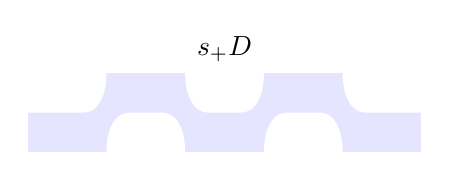
\begin{tikzpicture}[baseline=-0.65ex,scale=0.10]
        \node at (0, 8) {$s_+D$};
        \draw[fill=blue!10!white,draw=none] (-25, -5) rectangle (25, 5);
        \draw[fill=white, draw=none] (-15, -5) [in=left, out=up] to (-12, 0) -- (-8, 0) [in=up, out=right] to (-5, -5);
        \draw[fill=white, draw=none] (5, -5) [in=left, out=up] to (8, 0) -- (12, 0) [in=up, out=right] to (15, -5);
        \draw[fill=white, draw=none] (-5, 5) [in=left, out=down] to (-2, 0) -- (2, 0) [in=down, out=right] to (5, 5);
        \draw[fill=white, draw=none] (-25, 0) -- (-18, 0) [in=down, out=right] to (-15, 5) -- (-25, 5);
        \draw[fill=white, draw=none] ( 25, 0) -- ( 18, 0) [in=down, out=left] to ( 15, 5) -- ( 25, 5);
    \end{tikzpicture}
    \quad
    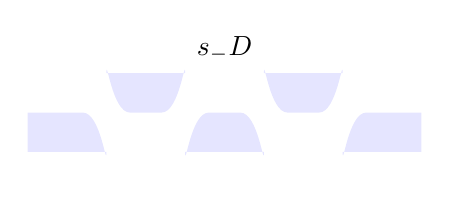
\begin{tikzpicture}[baseline=-0.65ex,scale=0.10]
        \node at (0, 8) {$s_-D$};
        \draw[fill=blue!10!white, draw=none] (-15, 5) [in=left, out=up] to (-12, 0) -- (-8, 0) [in=up, out=right] to (-5, 5);
        \draw[fill=blue!10!white, draw=none] (5, 5) [in=left, out=up] to (8, 0) -- (12, 0) [in=up, out=right] to (15, 5);
        \draw[fill=blue!10!white, draw=none] (-5, -5) [in=left, out=down] to (-2, 0) -- (2, 0) [in=down, out=right] to (5, -5);
        \draw[fill=blue!10!white, draw=none] (-25, 0) -- (-18, 0) [in=down, out=right] to (-15, -5) -- (-25, -5);
        \draw[fill=blue!10!white, draw=none] ( 25, 0) -- ( 18, 0) [in=down, out=left] to ( 15, -5) -- ( 25, -5);
    \end{tikzpicture}
\]

Zamknięte krzywe tworzące $s_+D$ są brzegami białych obszarów uszachowienia, 
podczas gdy te tworzące $s_-D$ stanowią brzeg czarnych obszarów.
Zauważmy jeszcze, że na każdym skrzyżowaniu są cztery różne czarne i białe obszary 
(nie mogą się spotkać w innych miejscach), gdyż diagram był zredukowany.

\begin{lemma}
Niech $D$ będzie spójnym diagramem splotu o $n$ skrzyżowaniach.
Wtedy mamy nierówność $|s_+D|+|s_-D|\le n+2$, z równością dla zredukowanego i alternującego $D$.
\end{lemma}

\begin{proof}
Skorzystamy z indukcji względem $n$.
Łatwo widać prawdziwość lematu dla $n = 0$.
Załóżmy, że jest on prawdziwy dla wszystkich diagramów o $n - 1$ skrzyżowaniach, następnie ustalmy diagram $D$ o $n$ skrzyżowaniach.

Wybierzmy skrzyżowanie z $D$. Można je wygładzić na dwa sposoby, jeden z nich daje spójny diagram $D'$.
Bez straty ogólności przyjmijmy, że jest to dodatnie wygładzenie.
Wtedy zachodzi $|s_+D'| = |s_+D|$, ale $|s_-D'|=|s_-D|\pm 1$, ponieważ $s_-D'$ powstaje z $s_-D$ przez zastąpienie pewnej części
$\MalyPrawyGladki$ z $\MalyLewyGladki$.
To rozrywa jedną krzywą na dwa kawałki lub scala dwie krzywe w jedną.
Teraz $|s_+D|+|s_-D| = |s_+D'|+|s_-D'|\pm 1 \le (n-1)+2\pm 1 \le n+2$ (pierwsza nierówność wynika z założenia indukcyjnego).

Załóżmy, że $D$ jest spójny, alternujący i zredukowany.
Musimy pokazać, że ostatnie dwie nierówności tak naprawdę są równościami.
Pierwsza wynika z tego, że $D'$ jest spójny, alternujący i zredukowany.
Z drugiej strony $|s_-D'|=|s_-D|-1$, ponieważ przejście od $s_-D$ do $s_-D'$ skleja dwa czarne obszary.
To pokazuje drugą równość i kończy dowód.
\[
    \begin{tikzpicture}[baseline=-0.65ex,scale=0.20]
    \begin{knot}[clip width=5] 
        \strand[semithick] (-5, 0) to (5, 0);
        \strand[semithick] (0, -5) to (0, 5);
        \draw[fill=blue!10!white,draw=none] (-5, -5) rectangle (0, 0);
        \draw[fill=blue!10!white,draw=none] ( 5,  5) rectangle (0, 0);
        \node at (0, -8) {$D$};
    \end{knot}
    \end{tikzpicture}
    \quad
    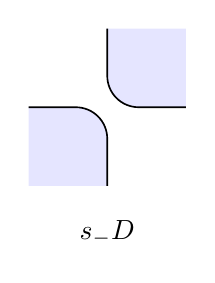
\begin{tikzpicture}[baseline=-0.65ex,scale=0.20]
        \draw[fill=blue!10!white, draw=none] (-5, 0) -- (-2, 0) [in=up, out=right] to (0, -2) -- (0, -5) -- (-5, -5);
        \draw[fill=blue!10!white, draw=none] (5, 0) -- (2, 0) [in=down, out=left] to (0, 2) -- (0, 5) -- (5, 5);
        \draw[semithick] (-5, 0) -- (-2, 0) [in=up, out=right] to (0, -2) -- (0, -5);
        \draw[semithick] (5, 0) -- (2, 0) [in=down, out=left] to (0, 2) -- (0, 5);
        \node at (0, -8) {$s_-D$};
    \end{tikzpicture}
    \quad
    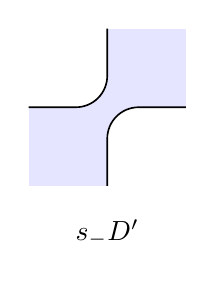
\begin{tikzpicture}[baseline=-0.65ex,scale=0.20]
        \draw[fill=blue!10!white, draw=none] (-5, -5) rectangle (5, 5);
        \draw[fill=white, draw=none] (5, 0) -- (2, 0) [in=up, out=left] to (0, -2) -- (0, -5) -- (5, -5);
        \draw[fill=white, draw=none] (-5, 0) -- (-2, 0) [in=down, out=right] to (0, 2) -- (0, 5) -- (-5, 5);
        \draw[semithick] (5, 0) -- (2, 0) [in=up, out=left] to (0, -2) -- (0, -5);
        \draw[semithick] (-5, 0) -- (-2, 0) [in=down, out=right] to (0, 2) -- (0, 5);
        \node at (0, -8) {$s_-D'$};
    \end{tikzpicture}
    \qedhere
\]
\end{proof}
\begin{lemma}
Niech $D$ będzie diagramem splotu o $n$ skrzyżowaniach.
Wtedy
\begin{enumerate}
\item $M \langle D \rangle \le n+2|s_+D|-2$
\item $m \langle D \rangle \ge -n-2|s_-D|+2$
\end{enumerate}
z równością, jeżeli $D$ jest alternujący, zredukowany i spójny.
\end{lemma}

\begin{proof}
Udowodnimy tylko pierwszą część, druga jest do niej podobna.
Oznaczymy przez $\langle D \mid s \rangle$ wielkość $(-A^{-2}-A^2)^{|sD|-1}A^{|s|}$.
Zauważmy, że $M\langle D|s\rangle=2|sD|+|s|-2$, 
a więc w szczególności $M\langle D|s_+\rangle=2|s_+D|+n-2$.
Gdyby udało się nam pokazać, że $M\langle D|s\rangle \le M\langle D|s_+\rangle$ 
dla wszystkich innych stanów $s$, dowód nierówności byłby zakończony.
Ale możemy znaleźć ciąg $s_+ = s_0$, $s_1$, \ldots, $s_r=s$, 
w którym $s_{i+1}$ powstaje z $s_i$ przez pojedynczą zmianę $+1$ na $-1$.

Teraz $|s_{i+1}|=|s_i|-2$, podczas gdy $|s_{i+1}D|=|s_iD|\pm 1$, 
ponieważ $s_{i+1}D$ uzyskujemy z $s_{i}D$ przez połączenie dwóch zamkniętych krzywych lub podział jednej zamkniętej krzywej na dwie części.
Zatem
\begin{align*}
    M \langle D \mid s_{i+1} \rangle & =
    2|s_{i+1}D|+|s_{i+1}|-2 \\ & =
    (2|s_iD| + |s_i| -2 ) + (\pm 2-2) \le
    M \langle D|s_i\rangle.
\end{align*}

Widać już, że $M\langle D \mid s\rangle =M\langle D \mid s_r\rangle \le\ldots\le M\langle D \mid s_0\rangle=M\langle D \mid s_+\rangle$.

Pokażemy teraz, że jeśli $D$ jest zredukowany, alternujący i spójny, to nierówność zamienia się w równość.
Będzie to wynikało z  $M\langle D|s\rangle<M\langle D| s_+\rangle$
dla $s\neq s_+$, jeżeli tylko powołamy się na powyższy argument.
Wystarczy ograniczyć się do tych $s$, które powstają z $s_+$ przez zmianę pojedynczego stanu $+1$ na $-1$.
Ale to już jest oczywiste, gdyż $sD$ otrzymujemy przez sklejenie dwóch białych obszarów $s_+ D$.
\end{proof}

Możemy wreszcie zająć się rozpiętością wielomianu Jonesa.

\begin{theorem}
Niech $L$ będzie zorientowanym splotem o spójnym diagramie $D$ z $n$ skrzyżowaniami.
Wtedy $\operatorname{span}(V(L)) \le n$, z równością dla zredukowanego i alternującego $D$.
\end{theorem}

\begin{proof}
    Pokażemy prawdziwość innego, równoważnego stwierdzenia: $\operatorname{span} \langle D\rangle\le 4n$ 
    z równością dla zredukowanego i alternującego $D$.
    Dwa poprzednie lematy mówią, że
    \begin{align*}
        \operatorname{span}\langle D\rangle 
        & = M\langle D\rangle - m\langle D\rangle \le (2|s_+D|+n-2)+(2|s_-D|+n-2) \\
        & = 2(|s_+D|+|s_- D|)+2n-4 \le 2(n+2)+2n-4 = 4n. \qedhere
    \end{align*}
\end{proof}

Jesteśmy już w stanie podać dowód twierdzenia \ref{taitjones} wspomnianego na początku sekcji.

\begin{proof}
    Założenia mówią nam, że $\operatorname{span} (V(L)) = n$.
    Gdyby istniał diagram o mniejszej liczbie skrzyżowań,
    mielibyśmy $\operatorname{span} (V(L)) < n$, co prowadzi do sprzeczności.
\end{proof}

Szukanie wielomianu Jonesa splotu bywa uciążliwe, 
jednak czasami możemy oszacować jego rozpiętość korzystając z następujących nierówności:

\begin{corollary}
    Niech $L$ będzie zorientowanym splotem ze spójnym diagramem $D$ o $n$ skrzyżowaniach.
    Wtedy
    \begin{align*}
        3w(D)-2|s_+D|+2-n & \le 4 m(V(L) \\
        3w(D)+2|s_-D|+n-2 & \ge 4 M(V(L)),
    \end{align*}
    z równością dla zredukowanego i alternującego $D$.
\end{corollary}

\begin{proof}
    Proste ćwiczenie.
\end{proof}

% Koniec podsekcji Rozpiętość i wielomian Jonesa


% Koniec sekcji Wielomian Jonesa
